\chapter{Architectural implementation}
\label{chap:archimpl}
 
In this chapter we will dig into the actual architectural implementation, seeing
all the problems related to it and how they were solved. We will show all the
various attemps made, and we will discussion about the technological issue and
changes we had to perform.

\section{First attempt}

In our first attempt we started building our infrastructure on top of Ubuntu
16.04 (for Openstack) and Ubuntu 18.04 (for Openbaton). Our main goal was to set
up Openstack as our VIM while setting Openbaton as our MANO. Then, Openbaton
would have Openstack registered as PoP, where TOSCA definition would be launched
on Openstack that, instead of deploying hypervisor based virtual machines, it
would have deployed container instances. The VNF lifecycles would have been
controller through an Element Management System (EMS), transmitting the various
VNF states via the message broker RabbitMQ. Is possible to see the interactions
between elements in a minimum schema available in
Figure~\ref{chap:archimpl:sec:fistattempt:img:schema1}.

\begin{figure}[t]
  \centering
  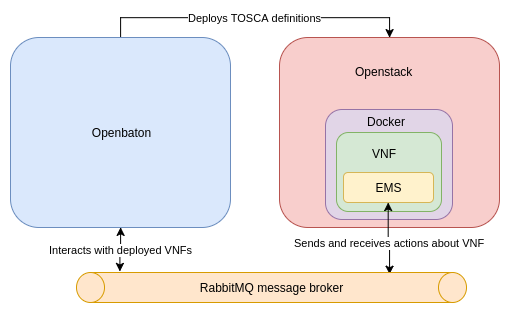
\includegraphics[scale=0.5]{Attempt1}
  \caption[Fist attempt components organization schema]{Fist attempt components
    organization schema. We can see how the main Openstack role is to deploy and
    manage the resources, while Openbaton has the role of maangement and
    orchestration. Finally, RabbitMQ sends and receives status update from the
    EMS for every VNF deployed.}
  \label{chap:archimpl:sec:fistattempt:img:schema1}
\end{figure}

\subsection{Adopting Openstack for container orchestration}

Our first step was to try to use Openstack to create a container orchestration. 
The reason behind this approach was simple: Openbaton, on paper, comes with an 
out-of-the-box support for Openstack. In fact, it natively supports Openstack 
PoPs, giving to us a great possibility to reuse the two frameworks and to ease 
the development phase of our software.
\subsubsection{Openstack for developers: Devstack}
Openstack is composed by modules, giving the possibility to the user who wants 
to install it to choose only the components it really needs. So the first thing 
we decided was to perform a selection of these modules between the 33 available 
in the installation page. The installation of this components span between 
multiple machines (nodes), therefore creating a whole cluster of resources. 
Since we considered too time-consuming to install Openstack in a distribuited 
manner, we considered to test first the developer version, called 
\emph{Devstack}. Devstack offers the possibility to install a subset of modules 
in the local machine, and to leverage a Openstack environment able to perform 
the same operations of the production-grade installation. Thus, we starting 
configurating the Devstack installation, installing first of all the Nova 
module, that is required to perform computer operations such as the launch of 
virtual machines, and lately we installed Tacker too.

\paragraph*{Taker}
\begin{figure}[h]
  \centering
  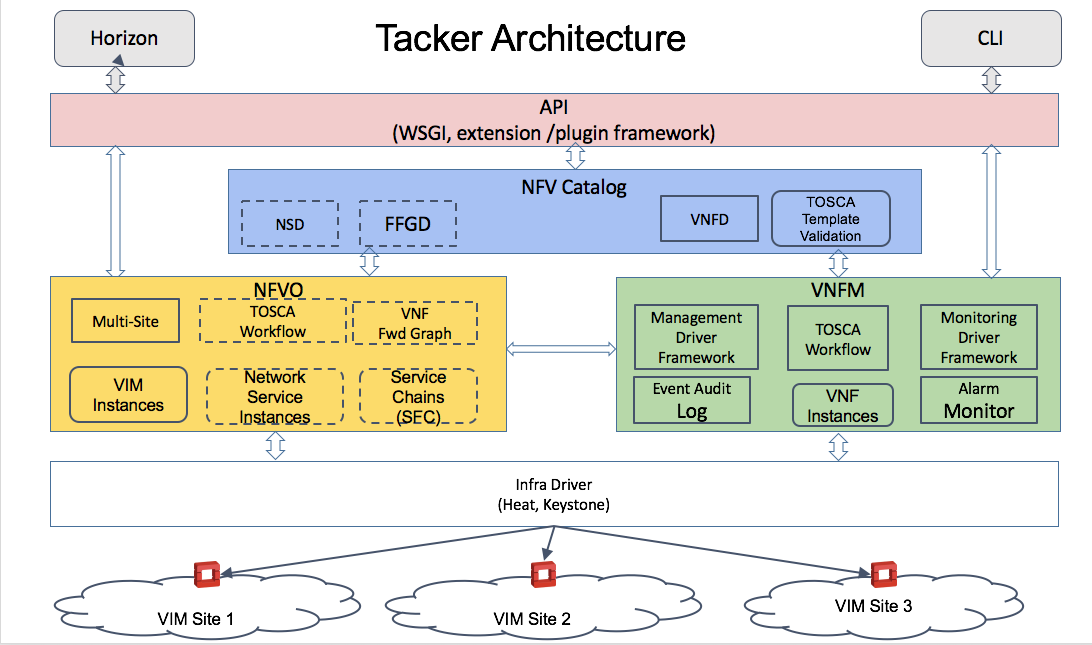
\includegraphics[scale=0.3]{tacker_architecture}
  \caption[Taker architecture schema]{Taker architecture
    schema~\cite{tackerOpenstackwiki}}
\end{figure}
Tacker is a VNFM and a NFVO. It is an official Openstack module, and it has the
ability to deploy, edit, stop and do periodic health checks VNF directly on it.
The develpers claim it has the possbility to make deployments to platforms
compatible with Openstack too. It supports VNF definition through the TOSCA
standard, and a proposal for SFC integration has been proposed in
2015~\cite{tackerOpenstackwiki}.

We sperimented Tacker to see if its functionalities were good enough to be
adopted in our testbed instead of Openbaton. Its complete integration with
Openstack, indeed, was the main reason for its testing. We felt like the product
was not fully ready to be used in a real deployment though, since it lacked of
options like SFC management and the fact that it only officially supported
Openstack and not other cloud platforms was another reason to prefer Openbaton
eventually.

\paragraph*{Devstack configuration}
The Openstack installation is not an easy one, particularly for newcomers, that 
have to deal with a great set of tools and not-always-clear instructions. Here 
we will describe how we managed to get a single-node deployment up and running.

First of all, Devstack needs a machine with at least 16GB of ram and 50GB of HD 
space.
We decided to install these components:
\begin{itemize}
 \item Keystone (for identity management)
 \item Object storage
 \item Compute
 \item Tacker (we tested this module to see is Openstack was a suitable VIM too)
\end{itemize}

Using Devstack is a simple operation, but the time required to reach a correct 
configuration is very high. In particular, it required from 20 minutes to 1 
hour to install Devstack we a particular configuration, without knowing if the 
final installation was working or not. This trial-and-error approach consumed a 
considerable amount of time, but it was the only possibility we had.

For testing purposes, and in order to better understanding the Openstack
functionalities, we configured a first version with Virtual Machine support
only.

\subsubsection{Openbaton installation}
\paragraph*{Openbaton configuration}
With Devstack ready to be used as NFVI, we started working on Openbaton.
Openbaton currently offers three ways to be deployed:
\begin{itemize}
  \item Normal installation. Openbaton offers official Ubuntu repositories that,
    added into the system, offer a very smooth installation via the
    \verb!aptitude! command line utility, with the only cons of having to wait
    for the automatic Openbaton download, installation and configuration;
  \item Using Vagrant. Vagrant is a software that helps the deployment of
    software, and it offers drivers to deploy virtual virtual machines too;
  \item Docker Compose. At the time of our study, the Docker Compose had three
    different configurations, based on the necessity of the user. A minimal,
    standard and full deployment were offered.
\end{itemize}

Now we are going to do a short description about every installation/deploy method.

\subparagraph*{Installation via repository}
The installation via repositories granted us the possibility to select only the
necessary parts we needed. The back of the medal of this approach was the
impossibility to automate it: in fact, during the installation proces user
interaction was required, that we were not able to write down in a scripted
fashion.

\subparagraph*{Deployment via Vagrant}
The deployment via Vagrant confirmed our expectations because it revealed to be
was always smooth. The downside of this approach was the lack of customization
and of component management. The possibility to remove or add Openbaton Modules
dynamically later become fundamental to us. On top of that, the Vagrant
deployment uses a hyperviso virtualization system (based on Virtual Box), in
contrast with our goal to build a fully container-based system.

\subparagraph*{Deployment via Docker Compose}
The deployment with Docker Compose turned out to be best of the three
possibilities. The Docker Compose configuration offered an unprecedented
configuration flexibility, with the possibility to deploy only selected modules.
On top of that, this method let us manage the Openbaton version freely, having
more control on update especially during the development of our components.
Additionally, using this Docker Compose configuration allowed us to seamlessly
integrate the monitoring tools Zabbix, in order to have the possibility to
graphically see the data fetch from Openbaton about the system state. Finally, a
Docker based solution seemed to be the best approach since all of our components
were meant to be put inside a Docker container.

\subsection{Docker integration in Openstack}

\begin{figure}[t]
  \centering
  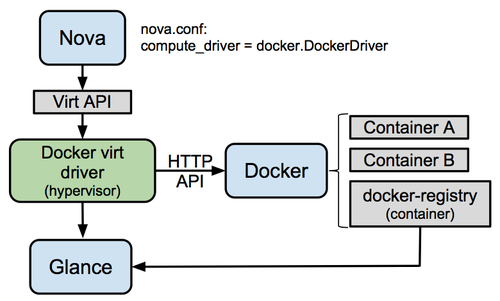
\includegraphics[scale=0.5]{dockeropenstackmodule}
  \caption[Docker module for Openstack working schema]{Docker module for Openstack
    working schema~\cite{openstackDockerModule}}
  \label{chap:archimpl:sec:fistattempt:img:dockeropnestackmodule}
\end{figure}

After the initial Openstack and Openbaton configuration we started making the
components talking to each other. First, we tried a simple \verb!iperf! data
transmission with two VNFs deployed by Openbaton as a common hypervisor-based
Openstack instances, as explained in~\cite{openbatonIperf}. With this test
completed, we started tinkering Openstack for using Docker containers instead of
traditional hypervisor instances. When we started developing this solution, we
adopted the Zun module, that aims to smoothly integrate Docker in Openstack.
Unfortunately, we were not able to make it properly work, in particular, it was
not possible to open desired ports on the Docker containers. This lead to the
impossibility to perform packet forwarding between VNFs. On top of that, we
found difficulties regarding the integration of Docker images in TOSCA
definitions and Openstack. These two issues are related: the TOSCA definition
does not have any keyword to specificate in any way that the image used for the
VNF definition is a Docker image, and Openstack, with the Zun plugin, at the
time of the implementation did not performed the image pull from any Docker
registry. The impossibility to easily set the containers ports and the lack of
some support in between the TOSCA definition and the Openstack Zun plugin pushed
us to drop Openstack as a possible solution and to start looking for another
valid VIM component.

\section{Second attempt}

After the failure to find a viable setting for Openstack, we decided to look
around for other solutions. We started studing proper Docker container
orchestrators that could offer all the features we needed: container lifecycle
management, scaling, healing and monitoring. We decided to pick two of the most
mature and famous ones: Docker Swarm and Kubenetes. The decision to study only
these two relies on their big community supporting them and the possibility to
easily found projects that used the forementioned frameworks.

\subsection{Docker Swarm}

\begin{figure}[t]
  \centering
  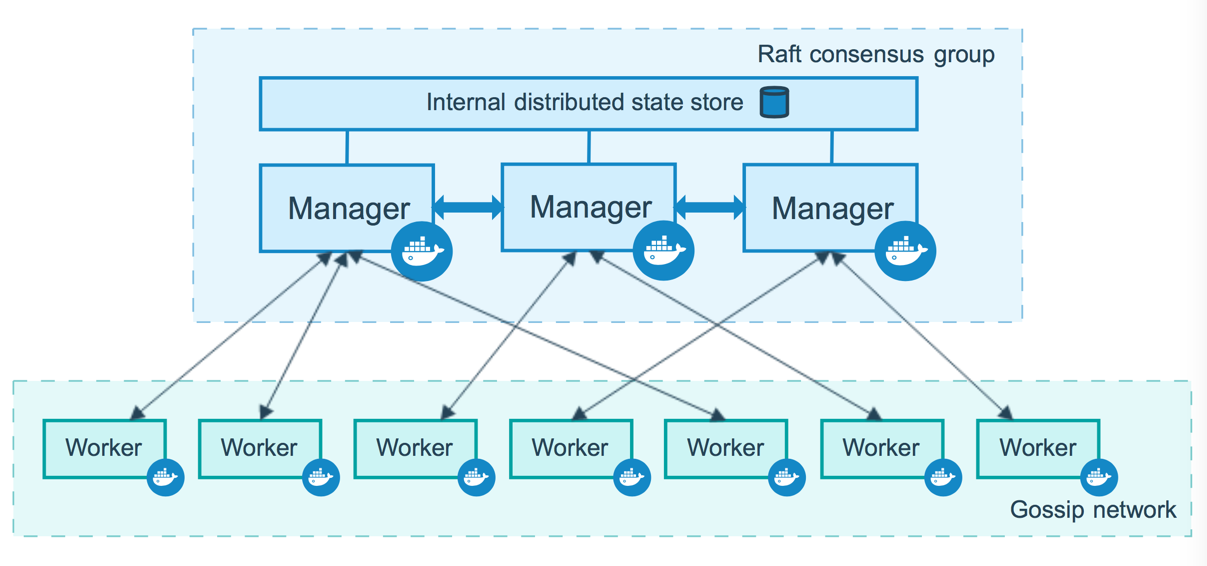
\includegraphics[scale=0.35]{swarm_diagram}
  \caption[Docker Swarm schema]{Docker Swarm schema~\cite{dockerSwarmWiki}.}
  \label{chap:archimpl:sec:secondattempt:img:dockerswarm}
\end{figure}

First we started playing with Docker Swarm. Docker Swarm is a product directly
made by the Docker Inc., so it seamlessly integrates with other Docker tools
such as Docker Compose. The installation and set-up is pretty straightforward,
and the configuration is almost automatically handed by Docker itself. The
minimum number of nodes in order to create a proper Docker Swarm cluster is of
free nodes, where one must be a manager node (designed to orchestrate the other
nodes in the cluster), while the other can be simple workers. Multiple managers
can coexist in the same cluster, as long as only one effectively operates. The
others act like backup manager in case the one orchestrating goes down for some
reason. The networking is given out-of-the box, and the same holds for
distributed persistence. While this for most of the uses cases can be considered
a pro, in our specific situation the impossibility to tweak the network
configuration was a cons, since it was important for us to have the full control
over the network, especially regarding the SFC implementation, explained better
in Chapter~\ref{chap:vnf_ns_impl}.

\subsection{Kubernetes}
Kubenetes, as already described in the technology section, is a orchestrator 
created by Google able to create a software abstraction from the underlying 
virtualization technology. This enables Kubernetes to create an integration 
with the Docker technology. Kubernetes has a architecture based on plug-ins, 
giving  the possibility to the users to change part of Kubernetes itself, such 
as the networking routing strategy or the persistence layer. With this 
flexibility Kubernetes offered to us what Docker Swarm was not able to give. 
Additionally, we had the possibility to set custom Domain Name System (DNS) 
lookups and distribute other internal components in order to avoid requests 
bottleneck.

\subsection{Kubernetes configuration}

\begin{figure}[t]
  \centering
  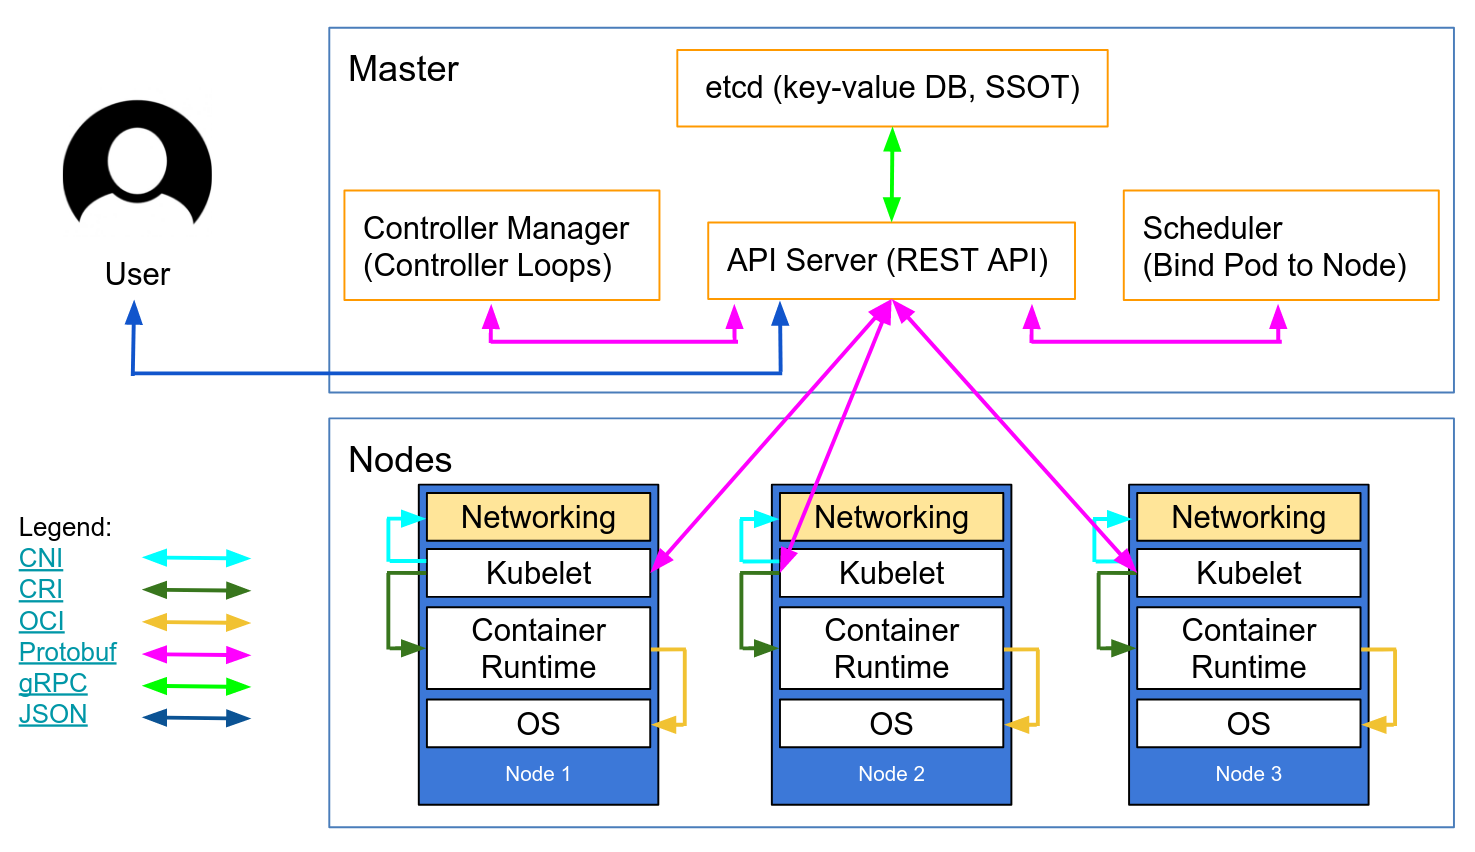
\includegraphics[scale=0.25]{kubernetes-control-plane}
  \caption[Kubernetes control plane schema]{Kubernetes control plane
    schema~\cite{k8scp}. It is possible to denothe important components in the
    Kubernetes Control plane. In this high-level component architecture the
    master keeps an internal database, \emph{etcd}, the entry point for the API
    Server and the Pod scheduler. The nodes instead contain the kubelet daemon,
    the container runtime and the networking configuration.}
  \label{chap:archimpl:sec:secondattempt:img:k8scp}
\end{figure}

Kubernetes does not have a minimum number of nodes in order to properly work.
Nonetheless, we decided to use a four node cluster configured in the following
way: three slaves nodes (also known as \emph{minions}) and one master node. The
Kubernetes version installed was the 1.11, enabling us to exploit new features
like a reworked DNS lookup system and new storage features\footnote{A full
  kubernetes log release can be found at:
  \url{https://kubernetes.io/blog/2018/06/27/kubernetes-1.11-release-announcement/}}.
We initially deployed from the internal Openstack of the University four nodes
with 4GB of RAM, 10 GB of SSD storage and 2 vCPUs on Ubuntu 16.04 machines. We
performed the installation using the official Kubernetes Repositories. After the
initial installation, we obtained a configuration similar to the one illustrated
in Figure~\ref{chap:archimpl:sec:secondattempt:img:k8scp}. In this figure is
possible to denote different components on the master node and on the minions,
which will be described.

\subsubsection{Master architecture}
\begin{description}
\item[API Server] Fist of all, the User interacts with an API Server located in
  the master node. This APIs are developed using the Swagger tools, ensuring
  consistency and uniformity. From the image, is possible to see that the API
  Server communicates with all the main components of the architecture.
\item[etcd] The \verb!etcd! component communicates via the gRCP protocol, a
  efficient Remote Procedure Call (RPC) protocol to serve data to the API
  Server. This component is a distributed key-value storage, and allows data to
  be shared in a reliable way across different machines~\cite{etcddatamodel}.
\item[Controller Manager] The Controller Manager is the main Kubernetes control
  loop, and its role is to periodically check the system health and integrity.
  It communicates with the API Server via the Protobuf protocol, a
  language-neutral, platform-neutral and extensible data serialization
  mechanism.
\item[Scheduler] The Scheduler regulates the Pods distribution in the minions,
  having a knowlege of the current cluster typologies and of the current
  resources available. On top of that, is able to handle hardware constraints,
  defined policy, and defined class of QoS.
\end{description}

All of the previously descripted components are hide beghind the API server,
which is the only components the final user can really interact with. The
protocol between the API server and the final user used is a common JSON data
object interchange. To make the Kubernetes more human-friendly, Kubernetes comes
with a command line interface (CLI) tool, called \verb!kubectl!, that allows to
easily perform deployments and admin operations on the cluster without having a
full knowlege of the official API.

\subsubsection{Minions architecture}

As referred in Figure~\ref{chap:archimpl:sec:secondattempt:img:k8scp}, the API
server interacts with the components located in the minion nodes. In the image
we can denote different modules.
\begin{description}
\item[Kubelet] The \verb!kubelet! daemon is the core component that runs in
  every minion, and \emph{de facto} acts like a local manager. It receives YAML
  or JSON definition from the API Server of Pod specifications (PodSpec) that
  have to be deployed in the node where is running. Then, its role is to ensure
  that the Pod deployed are up and healthy. This excludes possible
  intereferences with other virtualized deployments.
\item[Container Runtime] This runtime does not have to necessarily be based on
  Docker or a container-based technology, but it can be based on an hypervisor
  one, e.g. the KuberVirt project\footnote{Additional information about this
    project can be found at the following link: \url{https://kubevirt.io/}}. The
  container runtime performs the real Pods deployments.

  Communications between the container runtime and the Kubelet component are
  performed by the Container Runtime Interface (CRI), that consists of a series
  of specifications/requirements built on top of the Protobuf protocol API.
  Additionally, the Container Runtime has to communicate with the underlying OS,
  and this operation is performed using the Open Container Initiative (OCI)
  specification, which seeks to provide a standard on how to interact and run
  the container images on the OS.
\item[Networking] This part aims to provide to che container runtime network
  connectivity. The role of the networking module is to provide, over than the
  standard Internet connectivity, the possibility for Pods to see each other as
  a part of the same network, even if Pods could be dislocated in other minions
  working between different subnets or completely different networks. On top of
  that, dynamic port allocation has to be kept in consideration too. The
  Kubernetes networking model focus on three fundamental
  requirements~\cite{k8snetworkingwiki}:
  \begin{itemize}
  \item all containers have to communicate with all the other containers without
    NAT;
  \item all nodes have the possibility to communicate with all containers (and
    vice-versa) without NAT;
  \item the IP that a container sees itself as is the same IP that others see it
    as.
  \end{itemize}
  It is important to note that the IP addresses are at the Pod scope and not at
  the container one. Every Pod has in fact its own networking space. Containers
  inside a Pod can reach each other using the \verb!localhost! address. In
  Kubernetes, several networking implementation exists, like Flannel, Google
  Copmute Engine (GCE), Kube-route, Project Calico~\cite{k8snetworkingwiki}. For
  our deployment, we decided to use Flannel, that demonstrated to work without
  any particular configuration and to be mature enough to handle big workloads.

  The communications between this component and the Kubelet one is carried
  through the Cloud Native Interface (CNI) protocol, that consists of a set
  of specification and libraries for writing plugins to configure network
  interfaces in linux containers~\cite{cnigithub}.
\end{description}

\subsection{Openbaton integration}

\begin{figure}[t]
  \centering
  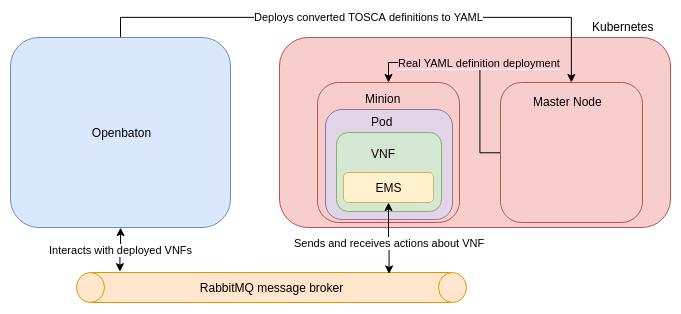
\includegraphics[scale=0.5]{Attempt2v1}
  \caption[Second attempt components organization schema]{Second attempt
    components organization schema. It is possible to see, differently from the
    first attempt, how now Kubernetes covers the old Openstack role and act as
    VIM, receiving YAML definitions in to the master node that will schedule the
    VNF in one of its minions.}
  \label{chap:archimpl:sec:secondattempt:img:schema1}
\end{figure}

After the Kubernetes configuration and installation, we started working for a
viable intergation between Kubernetes and Openbaton. Our first idea is the one
illustrated in Figure~\ref{chap:archimpl:sec:secondattempt:img:schema1}:
Openbaton, that had the TOSCA definitions, had to somehow convert these
definition in a suitable YAML for Kubernetes, that had in turn to elaborate it
and schedule to one minion in the cluster. The monitoring and management would
remain untouched, as we planned to create an image with the integrated EMS tools
that provided a seamless integration with Docker container. With this setting,
the only thing remained was to solve the issue of converting TOSCA definitions
in YAML one. The first thing we started thinking about was how to perform the
conversion. This topic was quite important because the TOSCA definition does not
really consider the possibility to have an alternative virtualization system
apart from the hypervisor one. This causes the TOSCA definition to be, in our
opinion, too much focused on the resources usage and regarding granularity
aspects such the deployment flavour and the kind of virtual link (concept that
does not really exsits in container based systems) to instatiate. Nonetheless,
we performed a mapping between most of the TOSCA keywords with some of the YAML
definition, in a way that a TOSCA configuration file was able to generate a
valid YAML deployment. After that, we started thinking instead who, in the
current architecture, had the task to perform this operation. Initially we
though that Kubernetes itself could have been a perfect candidate. From a
received TOSCA, a Kubernetes component should have validated and translated the
TOSCA definition to generate a YAML suitable to be finally submitted to the
Kubernetes API Server. Another feasible approach could have been to create a
Openbaton plugin in order to take the TOSCA to deploy and convert it before
submitting it to Kubernetes. This solution had great advantages in terms of
responsability separation: in this way only the MANO had to know, for a VIM
based on Kubernetes, that a conversion needed to be performed. From a Kuberentes
point-of-view, nothing would have changed, since all the configuration
conversion would have been performed by Openbaton.

\begin{figure}[t]
  \centering
  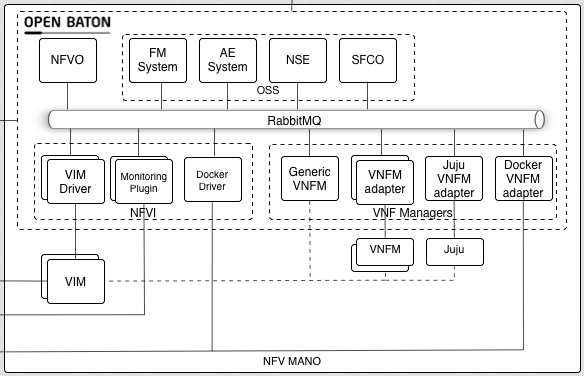
\includegraphics[scale=0.7]{OpenbatonMANO}
  \caption[Openbaton architecture components]{Openbaton architecture components,
    taken from~\cite{openbatondocumentation}.}
  \label{chap:archimpl:sec:secondattempt:img:openbatonMANO}
\end{figure}

We started inspecting the Openbaton framework, to identify possible modules
where the conversion should have taken place. We identified first the VIM
driver, that is the component that directly interacts with the VIM, and then the
VNFM, because we discovered there were programmatic dipendences between the two
Openbaton standard components. After we identified the VIM driver and the VNFM
as components to be rewritten and to be adapted to the Kubernetes VIM, we
studied the original components code. We discovered that regarding these
components the documentation was very poor, especially regarding the code. On
top of that, the program interfaces given by the develpers did not match our
expectations: we thought to find interfaces indipendent from the type of the
virtualization technology, instead, we found that they were strictly coupled
with frameworks like Openstack or cloud vendors like Google Compute engine or
Amazon AWS. These reasons, with the fact that after two weeks we were not able
to get any working prototype of VIM driver or VNFM we gave up, searching for
another solution.

\section{Second attempt - revision one}

The impossibility to develop a custom VIM driver and VNFM manager lead us to
search for an alternative solution. Then, we started work directly on the VIM.
The base approach was to create an API Server which in future an Openbaton
plugin could contact and simply deploy TOSCA definitions, interacting with a set
of RESTful API.

% TODO talk about the problems of mapping the TOSCA definition from Openbaton
% with the Kubernetes elements (which we actually solved), and talk about how we
% weren't able to develop a VNFM plugin for Openbaton, and describe how Harbor
% born from it.
